% Estudo numérico retrospectivo do DengueSphere — seções de métodos do estudo, resultados e discussão.
% Tabelas geradas por estudo/gerar_latex.py a partir de estudo/resultados/*.csv; figuras por estudo/analises.py.
% Compilar:  cd estudo/artigo && latexmk -pdf resultados.tex
\documentclass[11pt,a4paper]{article}
\usepackage[T1]{fontenc}
\usepackage[utf8]{inputenc}
\usepackage[brazilian]{babel}
\usepackage{lmodern}
\usepackage{microtype}
\usepackage[margin=2.3cm]{geometry}
\usepackage{amsmath}
\usepackage{siunitx}
\sisetup{group-separator={.}, output-decimal-marker={,}, group-minimum-digits=4}
\usepackage{booktabs}
\usepackage{adjustbox}
\usepackage{graphicx}
\usepackage[font=small,labelfont=bf]{caption}
\usepackage{subcaption}
\usepackage{float}
\usepackage[hidelinks]{hyperref}
\usepackage[capitalise,noabbrev,brazilian]{cleveref}
\graphicspath{{../figuras/}}
\setlength{\parskip}{0.35em}
\renewcommand{\arraystretch}{1.12}

\title{Avaliação numérica retrospectiva do DengueSphere:\\ 13 anos de casos de dengue no Recife (2013--2025)}
\author{}
\date{}

\begin{document}
\maketitle

\section{Desenho do estudo numérico}
\label{sec:desenho}

Como o DengueSphere ainda não foi adotado na rotina da vigilância municipal, a avaliação foi conduzida como um
\emph{estudo numérico retrospectivo}: o software foi reexecutado sobre o histórico de notificações e suas saídas foram
confrontadas com o que efetivamente ocorreu nas semanas seguintes. Todas as clusterizações usam as funções do próprio
serviço de processamento do DengueSphere (\texttt{executar\_clusterizacao} e \texttt{stability\_analysis}, DBSCAN com
métrica haversine), sem reimplementação.

\paragraph{Dados.} Foram utilizadas as notificações de dengue do SINAN publicadas no portal de dados abertos do Recife
(licença ODbL) para 2013--2025. Os 13 arquivos anuais apresentam dois esquemas de nomes de colunas, três formatos de CSV
e três codificações de caracteres, padronizados em uma única base. Incluíram-se residentes no Recife (IBGE 261160) com
classificação final confirmada --- códigos 1 a 4 da classificação vigente até 2014 (dengue clássico, dengue com
complicações, febre hemorrágica, síndrome do choque) e 10 a 12 da classificação revisada (dengue, dengue com sinais de
alarme, dengue grave). Descartados e inconclusivos foram excluídos da análise principal. A data de referência é a do
início dos sintomas (ou da notificação, quando ausente).

\paragraph{Geocodificação.} Os arquivos públicos não contêm coordenadas. Para geocodificar os \num{69681} registros não
descartados (\num{29043} pares únicos logradouro--bairro) sem violar os limites de uso do serviço Nominatim, a cascata
de geocodificação do DengueSphere (logradouro $\rightarrow$ bairro $\rightarrow$ não encontrado) foi reproduzida sobre
uma base local do OpenStreetMap: \num{18739} trechos de logradouros nomeados recortados pelos 94 polígonos de bairros
(219,3~km$^2$). Os nomes foram normalizados (abreviações, ordinais, números por extenso, caracteres corrompidos) e casados
por similaridade textual (\emph{token sort ratio} $\geq 85$). A concordância com o geocodificador original foi medida na
amostra de 2021 já processada pelo DengueSphere.

\paragraph{População.} Os denominadores vêm do Censo Demográfico 2022 do IBGE, usando a malha de setores censitários
com atributos (\num{2836} setores, \num{1488924} habitantes no Recife). A população de cada setor foi distribuída
entre as células de uma grade regular de 100~m na proporção da área de interseção (ponderação areal). A soma por bairro
reproduziu os totais publicados pelo IBGE com correlação de 0,9995 e diferença absoluta mediana de 1,9\%. A mesma
população de 2022 foi usada em todos os anos; a população do município variou pouco no período (cerca de $-3\%$
entre os Censos de 2010 e 2022). A \cref{fig:ponderacao} ilustra o procedimento.

\begin{figure}[htbp]
  \centering
  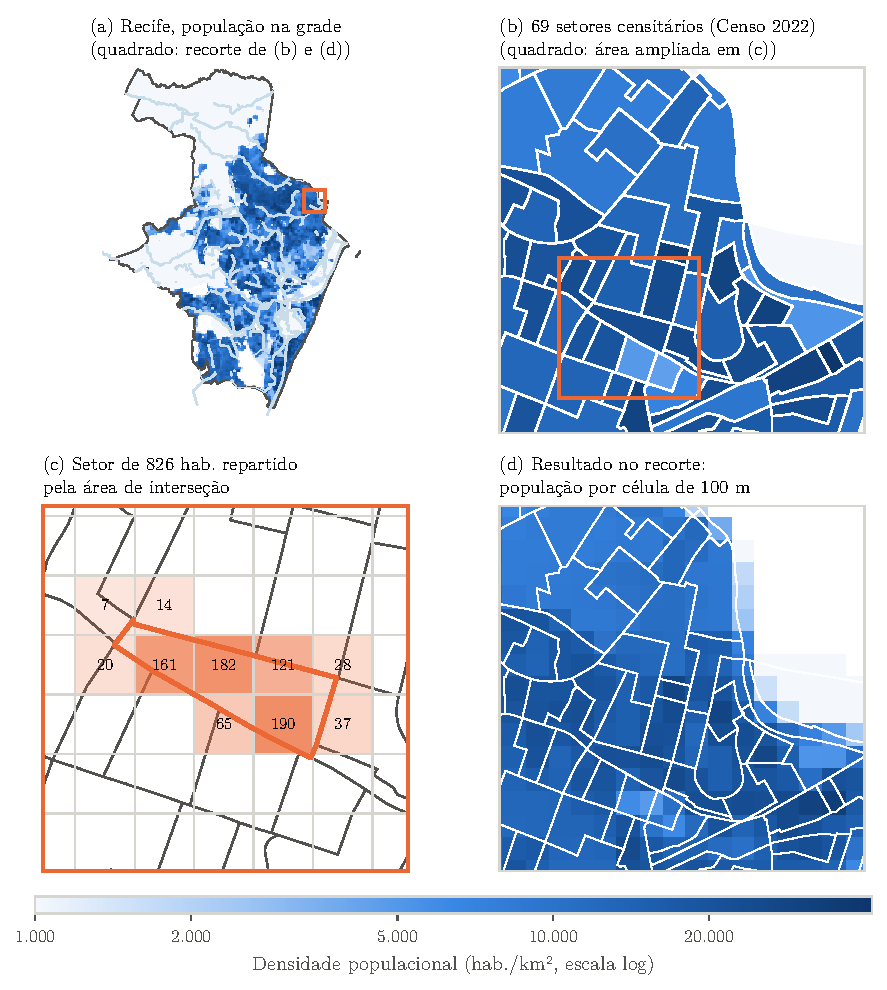
\includegraphics[width=0.95\linewidth]{fig12_ponderacao_areal.pdf}
  \caption{Distribuição da população do Censo 2022 na grade de 100~m por ponderação areal. (a) Resultado para todo o
  município. (b) Setores censitários de um recorte de 1,6~km na zona norte, coloridos pela densidade populacional.
  (c) Ampliação de um setor de 826 habitantes: cada célula recebe a fração da população proporcional à área do setor
  que ela cobre (números: habitantes atribuídos à célula; soma = 826). (d) População por célula no mesmo recorte, na
  mesma escala de cores de (b).}
  \label{fig:ponderacao}
\end{figure}

\paragraph{Janelas de análise.} A unidade de avaliação é a \emph{janela} de 4 semanas epidemiológicas de casos
geocodificados no nível de logradouro, que reproduz o uso pretendido do software (seleção de semanas recentes e
clusterização). As janelas foram estratificadas pelo nível de incidência: baixa ($<100$ casos), média (100--400) e alta
($>400$).

\paragraph{Métricas.} (i) \emph{Sensibilidade} aos parâmetros: número de clusters, proporção de ruído e silhueta na
grade $\varepsilon \in \{0{,}1;\,0{,}2;\,0{,}3;\,0{,}5;\,0{,}75;\,1{,}0\}$~km $\times$ \texttt{min\_samples}
$\in \{3, 5, 10, 15, 20\}$. (ii) \emph{Estabilidade}: índice de Rand ajustado (ARI) entre a solução de referência e soluções
com $\varepsilon \pm 10\%$, \texttt{min\_samples} $\pm 1$ e subamostras de 90\% dos casos. (iii) \emph{Validação
prospectiva}: a cada semana $t$, o DBSCAN é aplicado às semanas $t-3,\dots,t$; a área sinalizada é o conjunto de células
de 100~m a até $\varepsilon$ de um caso pertencente a algum cluster. Mede-se a captura (fração dos casos das semanas
$t+1,\dots,t+4$ dentro da área) e o \emph{Predictive Accuracy Index},
\begin{equation}
  \text{PAI} = \frac{\text{casos futuros na área}\,/\,\text{casos futuros}}{\text{área sinalizada}\,/\,\text{área do município}},
\end{equation}
em que PAI $=1$ equivale a uma escolha aleatória de áreas. Como áreas densamente povoadas tendem a ter mais casos
apenas por terem mais moradores, calculou-se também o PAI populacional,
\begin{equation}
  \text{PAI}_\text{pop} = \frac{\text{casos futuros na área}\,/\,\text{casos futuros}}{\text{população na área}\,/\,\text{população do município}},
\end{equation}
que vale 1 quando a área sinalizada tem o mesmo risco por habitante que a média da cidade. O DBSCAN é comparado com
quatro referências: estimativa de densidade kernel (KDE) com a mesma área; ranking de bairros por incidência (casos
por habitante) na janela; as células mais populosas com a mesma área, sem nenhuma informação sobre casos; e um
\emph{buffer} de todos os casos da janela sem clusterização. Os parâmetros foram escolhidos em 2013--2019 (treino) e avaliados em 2020--2025 (teste),
com comparação pareada por janela pelo teste de postos sinalizados de Wilcoxon. (iv) \emph{Persistência interanual}:
correlação de Spearman entre anos dos casos por célula de 500~m e da incidência por bairro. (v) \emph{Desempenho computacional}.

\section{Resultados}

\subsection{Base de dados e geocodificação}

Entre 2013 e 2025 foram registradas \num{110468} notificações de dengue de residentes no Recife, das quais \num{63347}
(57,3\%) foram confirmadas (\cref{tab:casos}). A série é dominada pela epidemia de 2015--2016, que concentra
\num{35659} confirmações (56,3\% do período), com pico de \num{1573} casos na semana epidemiológica 14 de 2015
(\cref{fig:curva}). Seguem-se 2021 (\num{7435} casos) e 2025 (\num{5066}). A incidência média foi de 327 casos por 100 mil habitantes
por ano, variando de 64 (2017) a \num{1583} por 100 mil (2015). O arquivo de 2014 termina em julho, o que produz uma
lacuna de cinco meses na série e subestima a incidência daquele ano.

\begin{figure}[htbp]
  \centering
  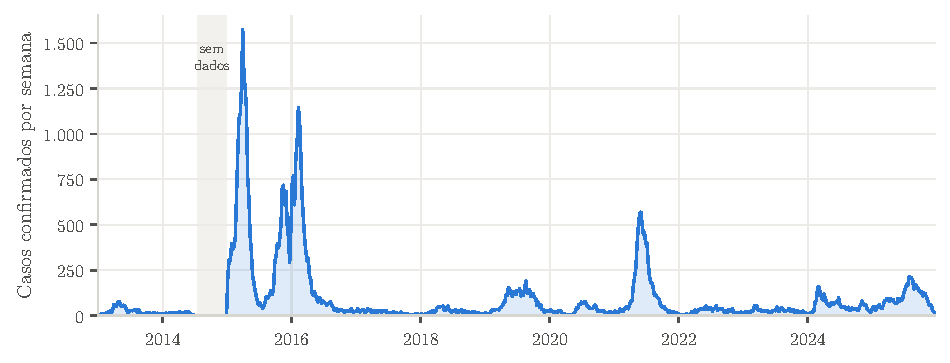
\includegraphics[width=\linewidth]{fig1_curva_epidemica.pdf}
  \caption{Casos confirmados de dengue por semana epidemiológica, Recife, 2013--2025. A faixa cinza indica o período sem
  dados no arquivo de 2014.}
  \label{fig:curva}
\end{figure}

\begin{table}[htbp]
\centering
\small
\caption{Notificações, casos confirmados, incidência e precisão da geocodificação por ano epidemiológico, Recife, 2013--2025.}
\label{tab:casos}
\begin{adjustbox}{max width=\linewidth}
\begin{tabular}{lrrrrrrrr}
\toprule
Ano & Notificados & Confirmados & Incid./100 mil & Rua (\%) & Bairro (\%) & Não enc. (\%) & Pico/sem. & SE do pico \\
\midrule
2013 & 3.262 & 1.304 & 87,6 & 85,4 & 14,6 & 0,0 & 77 & 18 \\
2014 & 1.159 & 363 & 24,4 & 85,7 & 14,3 & 0,0 & 24 & 20 \\
2015 & 34.675 & 23.576 & 1.583,4 & 80,8 & 18,6 & 0,5 & 1.573 & 14 \\
2016 & 18.505 & 12.083 & 811,5 & 81,6 & 17,3 & 1,0 & 1.144 & 6 \\
2017 & 2.445 & 955 & 64,1 & 81,9 & 18,1 & 0,0 & 41 & 2 \\
2018 & 2.686 & 1.207 & 81,1 & 81,3 & 18,2 & 0,5 & 53 & 19 \\
2019 & 7.309 & 4.102 & 275,5 & 81,3 & 17,6 & 1,0 & 190 & 34 \\
2020 & 3.619 & 1.544 & 103,7 & 81,0 & 18,5 & 0,5 & 79 & 30 \\
2021 & 10.977 & 7.435 & 499,4 & 82,4 & 17,6 & 0,0 & 569 & 22 \\
2022 & 2.795 & 1.291 & 86,7 & 83,5 & 16,3 & 0,2 & 55 & 31 \\
2023 & 3.502 & 1.414 & 95,0 & 86,0 & 13,9 & 0,1 & 57 & 11 \\
2024 & 10.483 & 3.007 & 202,0 & 87,8 & 12,0 & 0,2 & 160 & 10 \\
2025 & 9.051 & 5.066 & 340,2 & 87,0 & 12,9 & 0,1 & 215 & 31 \\
\midrule
\textbf{Total} & 110.468 & 63.347 & 327,3 & 82,4 & 17,1 & 0,5 & -- & -- \\
\bottomrule
\end{tabular}
\end{adjustbox}
\par\smallskip\begin{minipage}{0.95\linewidth}\footnotesize Notificados: residentes no Recife com data válida (qualquer classificação). Incidência: confirmados por 100 mil habitantes (Censo 2022, 1.488.924 hab.); na linha Total, média anual. Rua: geocodificado no nível de logradouro (no bairro informado, em bairro vizinho ou único na cidade). Bairro: ponto representativo do polígono do bairro. SE: semana epidemiológica. O arquivo de 2014 contém notificações apenas até julho.\end{minipage}
\end{table}


A geocodificação local posicionou 82,4\% dos casos confirmados no nível de logradouro, 17,1\% no ponto representativo do
bairro e deixou 0,5\% sem localização. A proporção no nível de rua variou de 80,8\% (2015) a 87,8\% (2024), com tendência
de melhora nos anos recentes (\cref{fig:geocod}).

\begin{figure}[htbp]
  \centering
  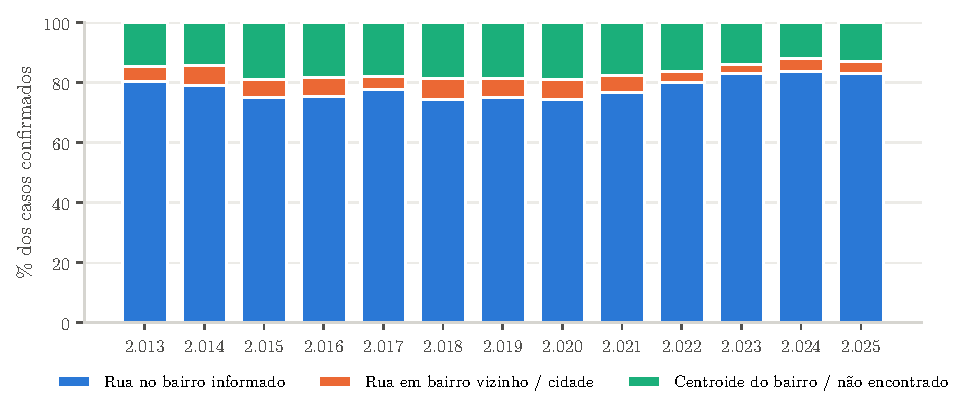
\includegraphics[width=\linewidth]{fig2_geocodificacao.pdf}
  \caption{Nível de precisão da geocodificação por ano.}
  \label{fig:geocod}
\end{figure}

Na amostra de 2021 processada pelo próprio DengueSphere (\cref{tab:validacao}), nos 809 casos em que ambos os métodos
encontraram o logradouro, a distância mediana entre as coordenadas foi de 56~m (percentil 90: 291~m), e 94,9\% ficaram a
até 500~m --- distância inferior ao menor $\varepsilon$ útil identificado adiante. A base local também resolveu no nível
de rua 148 casos que o Nominatim só localizou pelo bairro. No sentido inverso, os 47 casos marcados pelo Nominatim como
``rua sem bairro'' e que a base local situou no bairro informado ficaram a uma mediana de 5,5--6,1~km, provavelmente por
logradouros homônimos em outros pontos da cidade escolhidos erroneamente pelo serviço externo.

\begin{table}[htbp]
\centering
\small
\caption{Distância entre a geocodificação local (OSM) e a do DengueSphere (Nominatim) na amostra de 2021 ($n = 1.219$).}
\label{tab:validacao}
\begin{adjustbox}{max width=\linewidth}
\begin{tabular}{llrrrrrr}
\toprule
Nominatim & Local (OSM) & $n$ & Mediana (m) & P90 (m) & $\leq$250 m & $\leq$500 m & $\leq$1 km \\
\midrule
Endereço exato & Centroide do bairro & 60 & 298 & 1.103 & 35,0 & 65,0 & 86,7 \\
 & Rua no bairro & 794 & 55 & 278 & 88,5 & 95,1 & 98,7 \\
 & Rua em bairro vizinho & 11 & 158 & 489 & 63,6 & 90,9 & 100,0 \\
\addlinespace
Fallback bairro & Centroide do bairro & 61 & 276 & 840 & 42,6 & 88,5 & 90,2 \\
 & Rua no bairro & 148 & 471 & 1.056 & 25,0 & 52,7 & 87,2 \\
 & Rua em bairro vizinho & 9 & 1.279 & 1.872 & 0,0 & 0,0 & 44,4 \\
\addlinespace
Fallback bairro corrigido & Centroide do bairro & 9 & 513 & 1.609 & 0,0 & 33,3 & 88,9 \\
 & Rua no bairro & 31 & 1.156 & 2.371 & 6,5 & 16,1 & 41,9 \\
\addlinespace
Rua sem bairro & Centroide do bairro & 31 & 5.497 & 23.520 & 0,0 & 0,0 & 0,0 \\
 & Rua no bairro & 16 & 6.138 & 12.549 & 0,0 & 0,0 & 0,0 \\
 & Rua em bairro vizinho & 41 & 102 & 317 & 82,9 & 90,2 & 92,7 \\
\bottomrule
\end{tabular}
\end{adjustbox}
\par\smallskip\begin{minipage}{0.95\linewidth}\footnotesize Colunas $\leq$: percentual de casos a até a distância indicada. Categorias com $n < 9$ omitidas.\end{minipage}
\end{table}


\subsection{Padrões espaciais}

Os mapas de calor anuais da densidade de casos (\cref{fig:mapas}) mostram concentração recorrente na zona norte
(Água Fria, Casa Amarela, Nova Descoberta) e no extremo sudoeste (Cohab, Ibura), com focos variáveis no oeste (Várzea,
Iputinga) e na orla sul. Contagens absolutas, porém, refletem em parte onde mora mais gente. Ajustada pela população
(\cref{tab:incidencia,fig:bairros}), a incidência média anual variou de 99 a 993 casos por 100 mil habitantes entre os
72 bairros com pelo menos 5 mil moradores (mediana 326). Boa Viagem, segundo bairro em número absoluto de casos
(\num{2592}), tem incidência de 164 por 100 mil e ocupa a 62\textsuperscript{a} posição; Campina do Barreto, com
\num{1091} casos em \num{8452} habitantes, tem incidência seis vezes maior (993 por 100 mil). O mapa de risco relativo por bairro
(\cref{fig:rr}) confirma o padrão: nos anos epidêmicos, risco acima da média nos morros da zona norte e no sudoeste, e
abaixo da média na orla e em bairros como Boa Viagem, Espinheiro e Graças (121 a 164 casos por 100 mil).

\begin{figure}[htbp]
  \centering
  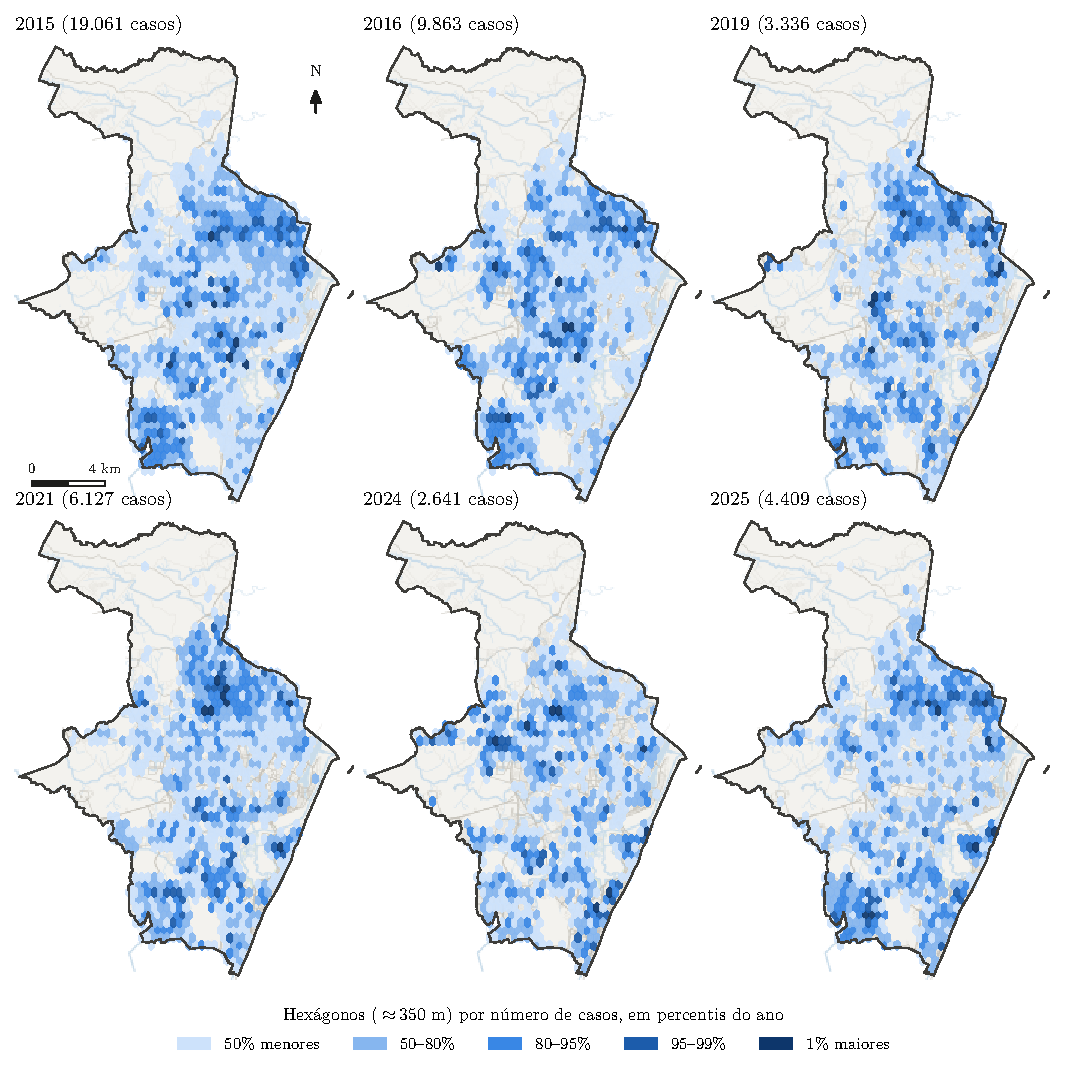
\includegraphics[width=0.92\linewidth]{fig8_mapas_calor_anuais.pdf}
  \caption{Mapas de calor da distribuição dos casos confirmados geocodificados no nível de logradouro nos seis anos com
  mais casos (os demais anos têm entre 311 e \num{1251} casos geocodificados; todos os 13 anos estão na
  \cref{fig:mapas_todos}). Cada hexágono (cerca de 350~m) é classificado pelo percentil do seu número de casos entre os hexágonos
  com casos no mesmo ano, o que torna os anos comparáveis apesar das diferenças de magnitude. Mapa base:
  OpenStreetMap (ruas, rios e mangues).}
  \label{fig:mapas}
\end{figure}

\begin{figure}[htbp]
  \centering
  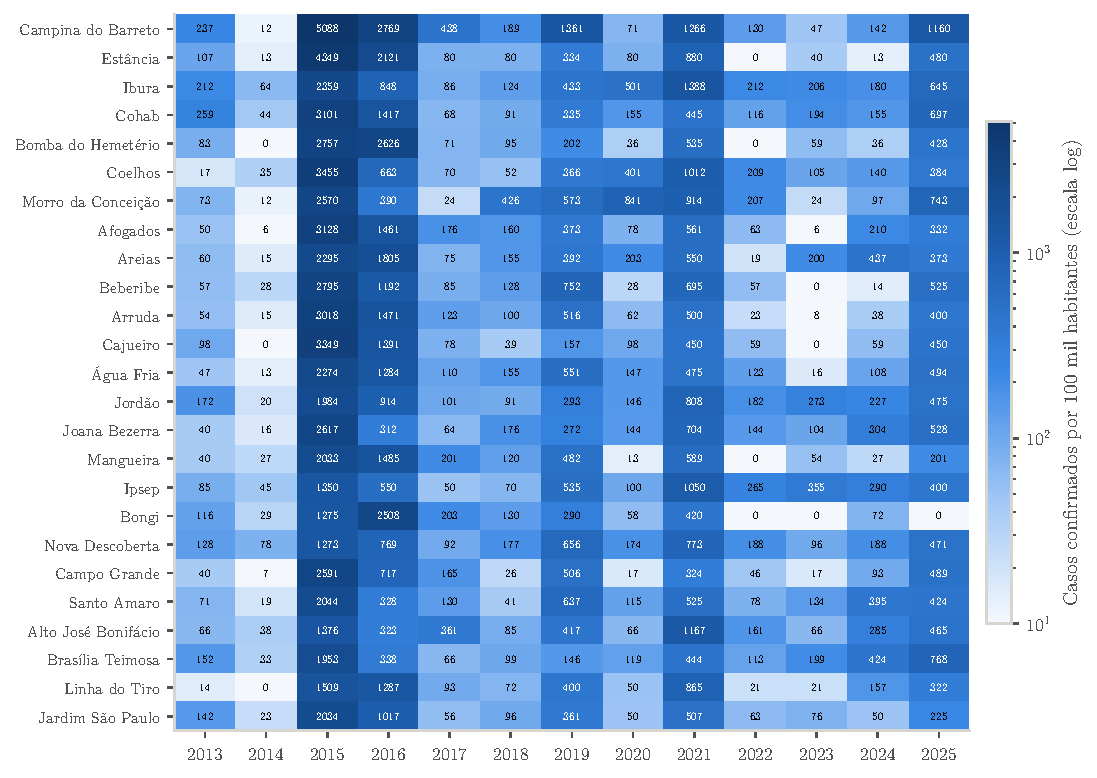
\includegraphics[width=0.95\linewidth]{fig10_bairro_ano.pdf}
  \caption{Mapa de calor da incidência anual de dengue (casos confirmados por 100 mil habitantes, escala logarítmica)
  nos 25 bairros de maior incidência média, entre os que têm pelo menos 5 mil moradores.}
  \label{fig:bairros}
\end{figure}

\begin{table}[htbp]
\centering
\small
\caption{Bairros com maior incidência média anual de dengue, 2013--2025.}
\label{tab:incidencia}
\begin{adjustbox}{max width=\linewidth}
\begin{tabular}{rlrrr}
\toprule
& Bairro & População (2022) & Casos & Incidência média anual/100 mil \\
\midrule
1 & Campina do Barreto & 8.452 & 1.091 & 992,9 \\
2 & Estância & 7.496 & 643 & 659,9 \\
3 & Ibura & 46.679 & 3.388 & 558,3 \\
4 & Cohab & 61.408 & 4.345 & 544,3 \\
5 & Bomba do Hemetério & 8.415 & 583 & 532,9 \\
6 & Coelhos & 5.731 & 396 & 531,5 \\
7 & Morro da Conceição & 8.209 & 566 & 530,4 \\
8 & Afogados & 31.901 & 2.107 & 508,1 \\
9 & Areias & 26.537 & 1.746 & 506,1 \\
10 & Beberibe & 7.047 & 448 & 489,0 \\
11 & Arruda & 12.988 & 822 & 486,8 \\
12 & Cajueiro & 5.106 & 318 & 479,1 \\
13 & Água Fria & 38.086 & 2.208 & 446,0 \\
14 & Jordão & 19.808 & 1.126 & 437,3 \\
15 & Joana Bezerra & 12.495 & 678 & 417,4 \\
\bottomrule
\end{tabular}
\end{adjustbox}
\par\smallskip\begin{minipage}{0.95\linewidth}\footnotesize Casos confirmados com bairro identificado (inclui casos localizados pelo centroide). Apenas bairros com pelo menos 5.000 habitantes. População estimada por ponderação areal dos setores censitários.\end{minipage}
\end{table}


\begin{figure}[htbp]
  \centering
  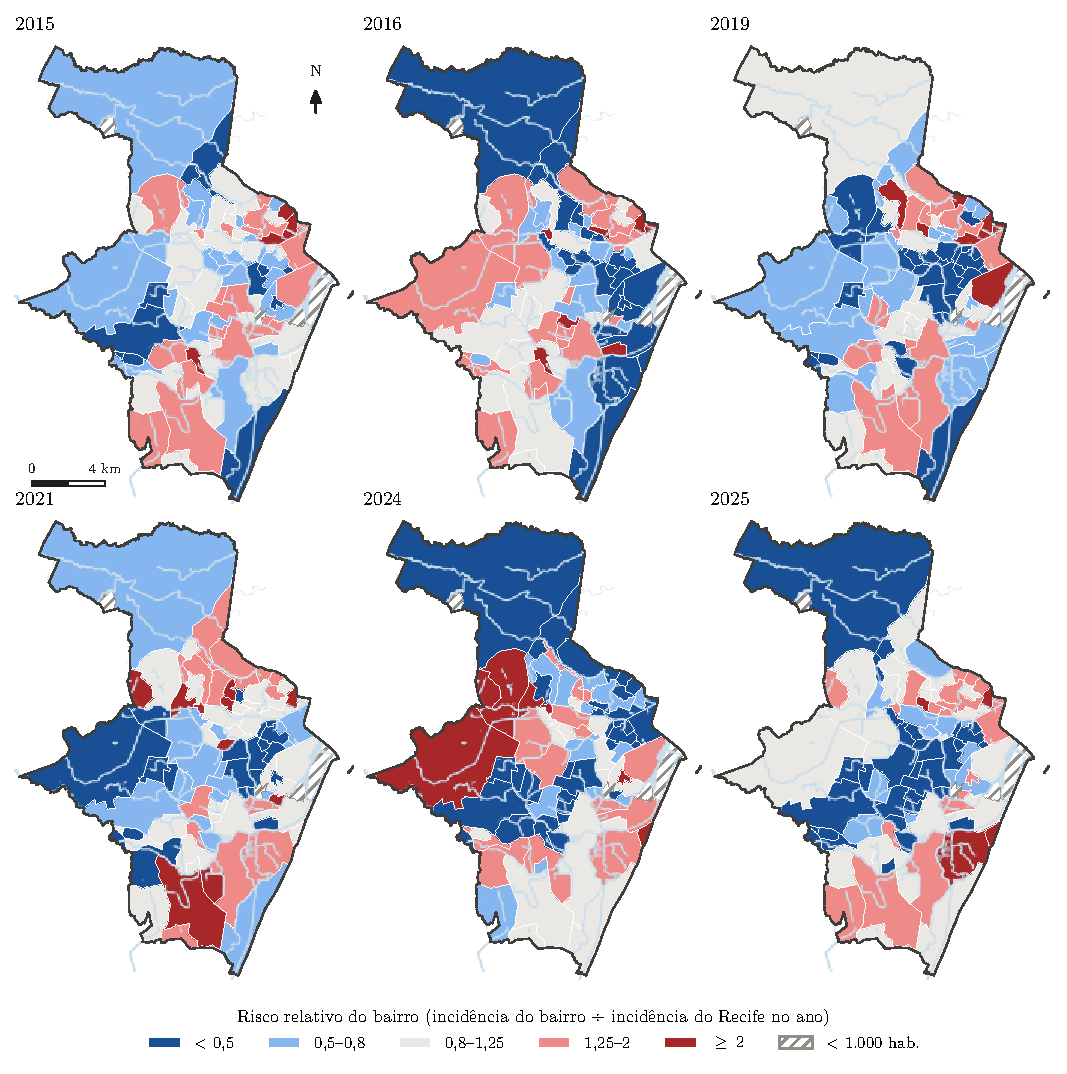
\includegraphics[width=0.92\linewidth]{fig11_risco_relativo_bairros.pdf}
  \caption{Risco relativo de dengue por bairro nos seis anos com mais casos (todos os anos na \cref{fig:rr_todos}): incidência do bairro (casos confirmados por
  habitante, Censo 2022) dividida pela incidência do Recife no mesmo ano. Vermelho: risco acima da média da cidade;
  azul: abaixo. Bairros com menos de \num{1000} habitantes (hachurados) foram omitidos por instabilidade da taxa.}
  \label{fig:rr}
\end{figure}

Entre anos consecutivos, a correlação de Spearman dos casos por célula de 500~m foi em média 0,52 (0,37 a 0,79;
\cref{tab:persistencia,fig:persistencia}). As células no decil superior de um ano, que ocupam cerca de 12\% das células
com casos, concentraram em média 26,2\% dos casos do ano seguinte, pouco mais que o dobro do esperado ao acaso. Em
incidência por bairro, a correlação entre anos consecutivos foi menor (média 0,35; negativa apenas entre 2014, ano
incompleto, e 2015). A persistência existe, mas é moderada: a distribuição espacial de um ano explica apenas parcialmente a do seguinte, o que
justifica uma ferramenta de detecção recorrente em vez de mapas de risco estáticos.

\begin{table}[htbp]
\centering
\small
\caption{Persistência espacial entre anos consecutivos.}
\label{tab:persistencia}
\begin{adjustbox}{max width=\linewidth}
\begin{tabular}{lrrrrr}
\toprule
& \multicolumn{2}{c}{Spearman} & & & \\
\cmidrule(lr){2-3}
Anos & Células 500 m & Incidência bairro & Jaccard top 10\% & Células top 10\% (\%) & Casos seguintes no top 10\% (\%) \\
\midrule
2013--2014 & 0,37 & 0,38 & 0,23 & 12,4 & 32,2 \\
2014--2015 & 0,38 & $-$0,17 & 0,11 & 12,2 & 18,8 \\
2015--2016 & 0,79 & 0,54 & 0,29 & 10,2 & 25,2 \\
2016--2017 & 0,45 & 0,26 & 0,27 & 10,2 & 26,5 \\
2017--2018 & 0,46 & 0,45 & 0,24 & 16,9 & 33,5 \\
2018--2019 & 0,58 & 0,44 & 0,20 & 13,7 & 28,0 \\
2019--2020 & 0,53 & 0,33 & 0,18 & 11,2 & 23,7 \\
2020--2021 & 0,51 & 0,38 & 0,24 & 12,9 & 26,3 \\
2021--2022 & 0,59 & 0,40 & 0,23 & 10,3 & 24,9 \\
2022--2023 & 0,46 & 0,38 & 0,30 & 12,4 & 30,8 \\
2023--2024 & 0,51 & 0,49 & 0,19 & 10,8 & 21,9 \\
2024--2025 & 0,60 & 0,30 & 0,20 & 11,3 & 23,4 \\
\midrule
Média & 0,52 & 0,35 & 0,22 & 12,0 & 26,2 \\
\bottomrule
\end{tabular}
\end{adjustbox}
\par\smallskip\begin{minipage}{0.95\linewidth}\footnotesize Células: contagem de casos por célula de 500 m. Incidência bairro: casos por habitante nos bairros com pelo menos 1.000 moradores. Top 10\%: células no decil superior de casos do ano anterior (empates incluídos).\end{minipage}
\end{table}


\begin{figure}[htbp]
  \centering
  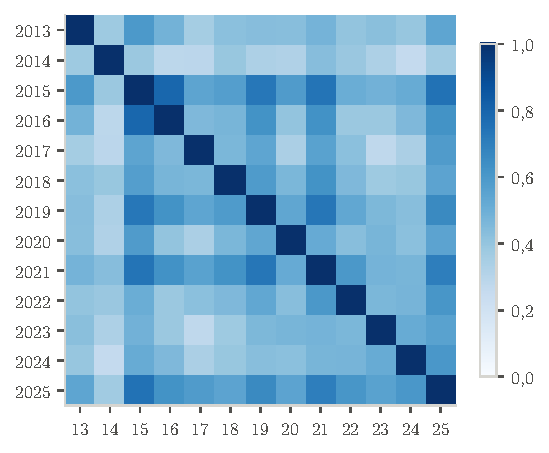
\includegraphics[width=0.55\linewidth]{fig7_persistencia.pdf}
  \caption{Mapa de calor da correlação de Spearman entre anos dos casos por célula de 500~m.}
  \label{fig:persistencia}
\end{figure}

\subsection{Sensibilidade aos parâmetros}

Foram avaliadas 154 janelas não sobrepostas de 4 semanas com pelo menos 30 casos (67 de baixa, 59 de média e 28 de alta
incidência). O comportamento do DBSCAN depende fortemente do nível de incidência (\cref{tab:sensibilidade,fig:sens}).
Com \texttt{min\_samples} = 10, no máximo 4\% das janelas de baixa incidência produziram algum cluster com $\varepsilon \leq
0{,}5$~km; com \texttt{min\_samples} = 3 e $\varepsilon = 0{,}3$~km, 73\%. Nas janelas de alta incidência, a mesma
configuração $\varepsilon = 0{,}3$~km e \texttt{min\_samples} = 3 gera uma mediana de 60 clusters e classifica só 20\% dos
casos como ruído. Ou seja, parâmetros fixos adequados a períodos epidêmicos silenciam o software em períodos
interepidêmicos, e vice-versa. A silhueta diminui com o aumento de $\varepsilon$ (de 0,95 a 0,48 com
\texttt{min\_samples} = 3), refletindo a fusão de agregados vizinhos em clusters maiores e menos compactos.

\begin{figure}[htbp]
  \centering
  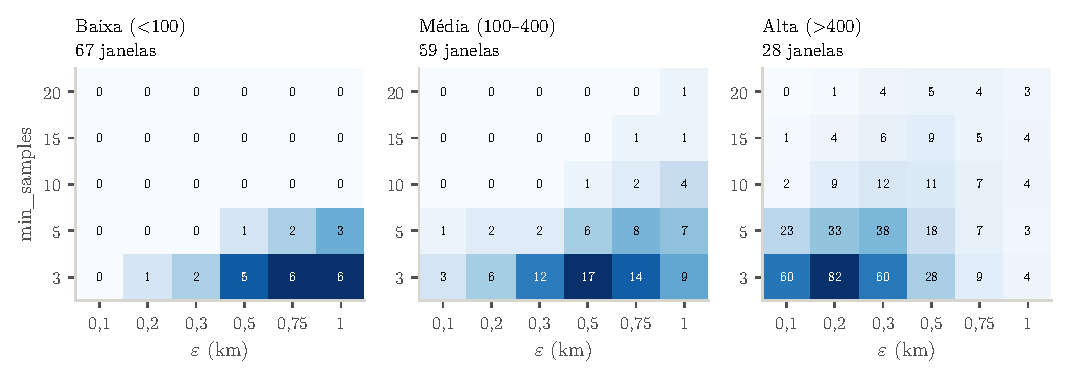
\includegraphics[width=\linewidth]{fig3_sensibilidade.pdf}
  \caption{Mapas de calor do número mediano de clusters por janela de 4 semanas na grade de parâmetros, por nível de
  incidência.}
  \label{fig:sens}
\end{figure}

\begin{table}[htbp]
\centering
\small
\caption{Sensibilidade do DBSCAN aos parâmetros, por nível de incidência da janela de 4 semanas (mediana [IIQ]).}
\label{tab:sensibilidade}
\begin{adjustbox}{max width=\linewidth}
\begin{tabular}{llrrrr}
\toprule
& eps (km) & min\_samples & Nº de clusters & Ruído (\%) & Janelas c/ cluster (\%) \\
\midrule
\multicolumn{6}{l}{\textit{Incidência baixa ($<$100); 67 janelas}} \\
 & 0,20 & 3 & 1 [0--2] & 95 [90--100] & 61 \\
 & 0,20 & 5 & 0 [0--0] & 100 [100--100] & 12 \\
 & 0,20 & 10 & 0 [0--0] & 100 [100--100] & 3 \\
 & 0,30 & 3 & 2 [0--3] & 90 [82--100] & 73 \\
 & 0,30 & 5 & 0 [0--0] & 100 [100--100] & 21 \\
 & 0,30 & 10 & 0 [0--0] & 100 [100--100] & 3 \\
 & 0,50 & 3 & 5 [2--6] & 71 [61--85] & 91 \\
 & 0,50 & 5 & 1 [0--1] & 93 [86--100] & 57 \\
 & 0,50 & 10 & 0 [0--0] & 100 [100--100] & 4 \\
 & 0,75 & 3 & 6 [4--8] & 49 [42--59] & 99 \\
 & 0,75 & 5 & 2 [1--3] & 76 [64--90] & 79 \\
 & 0,75 & 10 & 0 [0--0] & 100 [100--100] & 15 \\
\addlinespace
\multicolumn{6}{l}{\textit{Incidência média (100--400); 59 janelas}} \\
 & 0,20 & 3 & 6 [3--16] & 81 [71--90] & 100 \\
 & 0,20 & 5 & 2 [0--4] & 94 [86--100] & 71 \\
 & 0,20 & 10 & 0 [0--0] & 100 [98--100] & 25 \\
 & 0,30 & 3 & 12 [6--23] & 67 [52--76] & 100 \\
 & 0,30 & 5 & 2 [1--6] & 87 [77--95] & 88 \\
 & 0,30 & 10 & 0 [0--1] & 100 [91--100] & 41 \\
 & 0,50 & 3 & 17 [12--24] & 42 [25--50] & 100 \\
 & 0,50 & 5 & 6 [4--14] & 67 [46--76] & 98 \\
 & 0,50 & 10 & 1 [0--2] & 89 [80--100] & 63 \\
 & 0,75 & 3 & 14 [12--16] & 19 [10--27] & 100 \\
 & 0,75 & 5 & 8 [6--10] & 37 [21--54] & 100 \\
 & 0,75 & 10 & 2 [1--6] & 75 [52--91] & 85 \\
\addlinespace
\multicolumn{6}{l}{\textit{Incidência alta ($>$400); 28 janelas}} \\
 & 0,20 & 3 & 82 [42--150] & 37 [20--50] & 100 \\
 & 0,20 & 5 & 33 [18--81] & 56 [34--74] & 100 \\
 & 0,20 & 10 & 9 [2--28] & 78 [64--94] & 86 \\
 & 0,30 & 3 & 60 [43--79] & 20 [8--30] & 100 \\
 & 0,30 & 5 & 38 [22--52] & 37 [17--54] & 100 \\
 & 0,30 & 10 & 12 [5--34] & 61 [34--82] & 96 \\
 & 0,50 & 3 & 28 [21--33] & 5 [2--11] & 100 \\
 & 0,50 & 5 & 18 [16--21] & 13 [3--21] & 100 \\
 & 0,50 & 10 & 11 [9--14] & 31 [13--51] & 100 \\
 & 0,75 & 3 & 9 [5--13] & 1 [0--3] & 100 \\
 & 0,75 & 5 & 7 [4--11] & 3 [1--7] & 100 \\
 & 0,75 & 10 & 7 [5--9] & 10 [2--23] & 100 \\
\bottomrule
\end{tabular}
\end{adjustbox}
\par\smallskip\begin{minipage}{0.95\linewidth}\footnotesize Janelas de 4 semanas não sobrepostas com ao menos 30 casos geocodificados no nível de rua. IIQ: intervalo interquartil.\end{minipage}
\end{table}


\subsection{Estabilidade dos agrupamentos}

As soluções foram estáveis a perturbações de $\pm10\%$ em $\varepsilon$ (ARI mediano de 0,79 a 0,91) e à remoção
aleatória de 10\% dos casos (ARI de 0,91 a 0,93) em todas as configurações (\cref{tab:estabilidade}). A estabilidade a
\texttt{min\_samples} $\pm 1$ é alta para \texttt{min\_samples} = 10 (0,91--0,94), mas cai para 0,50--0,82 quando
\texttt{min\_samples} = 3. Nesse caso a perturbação representa uma variação relativa de 33\%, e com
\texttt{min\_samples} = 2 qualquer par de casos próximos forma um cluster. Em resumo, as áreas detectadas não
dependem de um ajuste fino dos parâmetros nem de casos individuais.

\begin{table}[htbp]
\centering
\small
\caption{Estabilidade dos agrupamentos: ARI mediano entre a solução de referência e a solução perturbada.}
\label{tab:estabilidade}
\begin{adjustbox}{max width=\linewidth}
\begin{tabular}{rrrrrrrr}
\toprule
eps (km) & min\_samples & Janelas & eps $\times$0,9 & eps $\times$1,1 & min\_samples $-$1 & min\_samples $+$1 & Subamostra 90\% \\
\midrule
0,20 & 3 & 128 & 0,90 & 0,89 & 0,50 & 0,65 & 0,93 \\
0,20 & 5 & 78 & 0,88 & 0,91 & 0,78 & 0,76 & 0,91 \\
0,20 & 10 & 41 & 0,88 & 0,90 & 0,93 & 0,91 & 0,92 \\
0,30 & 3 & 136 & 0,89 & 0,88 & 0,52 & 0,65 & 0,92 \\
0,30 & 5 & 94 & 0,87 & 0,89 & 0,79 & 0,81 & 0,92 \\
0,30 & 10 & 53 & 0,86 & 0,88 & 0,93 & 0,93 & 0,93 \\
0,50 & 3 & 148 & 0,86 & 0,86 & 0,61 & 0,68 & 0,92 \\
0,50 & 5 & 124 & 0,83 & 0,86 & 0,79 & 0,77 & 0,92 \\
0,50 & 10 & 68 & 0,84 & 0,80 & 0,91 & 0,94 & 0,93 \\
0,75 & 3 & 153 & 0,83 & 0,86 & 0,82 & 0,79 & 0,93 \\
0,75 & 5 & 140 & 0,80 & 0,88 & 0,80 & 0,80 & 0,92 \\
0,75 & 10 & 88 & 0,79 & 0,87 & 0,93 & 0,94 & 0,93 \\
\bottomrule
\end{tabular}
\end{adjustbox}
\par\smallskip\begin{minipage}{0.95\linewidth}\footnotesize ARI: índice de Rand ajustado (1 = partições idênticas). Perturbações de parâmetros calculadas com \texttt{stability\_analysis} do DengueSphere; subamostra: 10 réplicas por janela, ARI sobre os casos retidos. Excluídas as janelas sem cluster na referência, em que o ARI seria 1 trivialmente.\end{minipage}
\end{table}


\subsection{Validação prospectiva}

Foram avaliadas 593 janelas semanais (308 no treino e 285 no teste). Na grade de parâmetros (\cref{tab:grade,fig:grade})
há um compromisso claro entre concentração e cobertura. Configurações restritivas ($\varepsilon = 0{,}2$~km,
\texttt{min\_samples} = 10) atingem PAI mediano de 9,8 no teste, mas só emitem alerta em 22\% das janelas.
Configurações permissivas ($\varepsilon = 0{,}75$~km, \texttt{min\_samples} = 3) capturam 61\% dos casos futuros, porém
com PAI de 2,3. Pelo critério definido no treino (maior PAI entre as configurações com alerta em $\geq 80\%$ das
janelas), foi selecionada a configuração $\varepsilon = 0{,}3$~km e \texttt{min\_samples} = 3.

\begin{figure}[htbp]
  \centering
  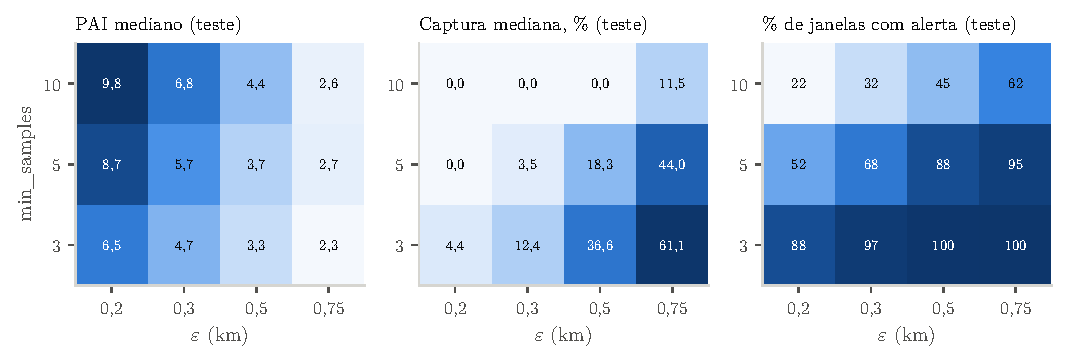
\includegraphics[width=\linewidth]{fig9_pai_grade_parametros.pdf}
  \caption{Mapas de calor do desempenho prospectivo do DBSCAN no período de teste (2020--2025): PAI mediano (janelas com
  alerta), captura mediana dos casos das 4 semanas seguintes e proporção de janelas com ao menos um cluster.}
  \label{fig:grade}
\end{figure}

\begin{table*}[htbp]
\centering
\small
\caption{Desempenho prospectivo do DBSCAN na grade de parâmetros (medianas por janela). Em negrito, a configuração escolhida no treino.}
\label{tab:grade}
\begin{adjustbox}{max width=\linewidth}
\begin{tabular}{rrrrrrrrrrr}
\toprule
& & \multicolumn{4}{c}{Treino (2013--2019)} & \multicolumn{5}{c}{Teste (2020--2025)} \\
\cmidrule(lr){3-6}\cmidrule(lr){7-11}
eps & min\_s. & Alerta \% & Capt. \% & Área \% & PAI & Alerta \% & Capt. \% & Área \% & PAI & PAI$_\text{pop}$ \\
\midrule
0,20 & 3 & 77 & 4,9 & 0,33 & 6,76 & 88 & 4,4 & 0,43 & 6,53 & 2,64 \\
0,20 & 5 & 53 & 0,0 & 0,10 & 7,74 & 52 & 0,0 & 0,08 & 8,75 & 3,20 \\
0,20 & 10 & 35 & 0,0 & 0,00 & 6,94 & 22 & 0,0 & 0,00 & 9,76 & 3,31 \\
\textbf{0,30} & \textbf{3} & \textbf{85} & \textbf{12,3} & \textbf{1,31} & \textbf{4,86} & \textbf{97} & \textbf{12,4} & \textbf{1,74} & \textbf{4,73} & \textbf{2,14} \\
0,30 & 5 & 62 & 3,1 & 0,31 & 5,59 & 68 & 3,5 & 0,43 & 5,73 & 2,47 \\
0,30 & 10 & 39 & 0,0 & 0,00 & 5,20 & 32 & 0,0 & 0,00 & 6,81 & 2,81 \\
0,50 & 3 & 94 & 31,1 & 6,45 & 3,13 & 100 & 36,6 & 8,75 & 3,29 & 1,66 \\
0,50 & 5 & 78 & 14,6 & 2,18 & 3,64 & 88 & 18,3 & 3,15 & 3,71 & 1,79 \\
0,50 & 10 & 46 & 0,0 & 0,00 & 3,78 & 45 & 0,0 & 0,00 & 4,40 & 2,29 \\
0,75 & 3 & 99 & 54,6 & 20,45 & 2,38 & 100 & 61,1 & 24,02 & 2,33 & 1,36 \\
0,75 & 5 & 88 & 37,6 & 10,02 & 2,66 & 95 & 44,0 & 13,92 & 2,67 & 1,52 \\
0,75 & 10 & 58 & 10,6 & 2,31 & 2,65 & 62 & 11,5 & 2,46 & 2,56 & 1,54 \\
\bottomrule
\end{tabular}
\end{adjustbox}
\par\smallskip\begin{minipage}{0.95\linewidth}\footnotesize Alerta: \% de janelas em que o DBSCAN encontrou ao menos um cluster. Captura: \% dos casos das 4 semanas seguintes dentro da área sinalizada (zero quando não há alerta). Área: \% da área do município (219,3 km$^2$). PAI = Captura/Área e PAI$_\text{pop}$ = Captura/\% da população, calculados apenas nas janelas com alerta. Critério de escolha: maior PAI mediano no treino entre as configurações com alerta em $\geq$80\% das janelas.\end{minipage}
\end{table*}


Com essa configuração, no período de teste, as áreas sinalizadas pelo DengueSphere ocuparam em mediana 1,8\% do
município e capturaram 13,3\% dos casos das 4 semanas seguintes: PAI mediano de 4,73 (IIQ 3,54--7,97), quase cinco vezes
o esperado ao acaso (\cref{tab:comparacao,fig:pai}). O desempenho no teste foi equivalente ao do treino (PAI 4,86), sem
sinal de sobreajuste.

Parte dessa concentração, porém, decorre da densidade demográfica: as células mais populosas da cidade, escolhidas sem
nenhuma informação sobre casos e com a mesma área, já alcançam PAI de 3,22. O PAI populacional isola esse efeito. As
áreas sinalizadas pelo DBSCAN abrigavam 4,1\% da população e receberam 13,3\% dos casos seguintes, um risco por
habitante 2,14 vezes maior que a média do Recife (IIQ 1,58--3,42; treino 2,13). Para as células mais populosas, esse
valor foi de 0,70: as áreas mais densas da cidade têm \emph{menos} casos por habitante que a média. O DBSCAN superou
essa referência populacional em 96,8\% das janelas de teste ($\Delta$PAI$_\text{pop}$ $+1{,}41$; $p<0{,}001$), o que
mostra que o software identifica risco além do que a distribuição da população explica (\cref{tab:pareada}).

Na comparação com as demais referências, os dois PAIs contam histórias complementares. Por área, o DBSCAN superou o
ranking de bairros por incidência em 91,3\% das janelas ($\Delta$PAI $+2{,}40$) e o \emph{buffer} de todos os casos em
88,8\% ($+1{,}49$), ambos com $p<0{,}001$. Por habitante, a vantagem sobre o \emph{buffer} se mantém (83,8\% das
janelas; $+0{,}55$), mas o ranking de bairros por incidência alcança risco por habitante equivalente (PAI$_\text{pop}$
2,13 contra 2,14; $p = 0{,}29$). Ou seja, priorizar bairros inteiros pela incidência atinge a mesma proporção de
casos por morador visitado, mas exige cobrir quase o dobro da área (3,3\% contra 1,8\% do município). A KDE de mesma
área foi ligeiramente superior ao DBSCAN nas duas métricas ($\Delta$PAI $-0{,}36$; $\Delta$PAI$_\text{pop}$ $-0{,}10$).

\begin{figure}[htbp]
  \centering
  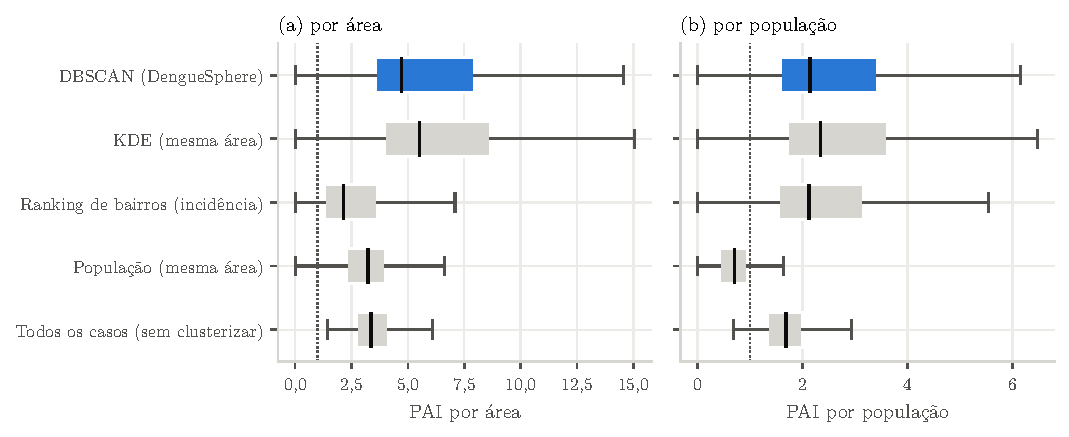
\includegraphics[width=\linewidth]{fig4_pai_metodos.pdf}
  \caption{Distribuição, por janela do período de teste (2020--2025), do PAI por área (a) e por população (b) na
  previsão dos casos das 4 semanas seguintes ($\varepsilon = 0{,}3$~km, \texttt{min\_samples} = 3). A linha pontilhada
  (valor 1) corresponde, em (a), à seleção aleatória de áreas e, em (b), ao risco médio por habitante da cidade.}
  \label{fig:pai}
\end{figure}

\begin{table*}[htbp]
\centering
\small
\caption{Validação prospectiva: DBSCAN ($\varepsilon$ = 0,3 km, min\_samples = 3) e métodos de referência na previsão dos casos das 4 semanas seguintes (medianas por janela com alerta).}
\label{tab:comparacao}
\begin{adjustbox}{max width=\linewidth}
\begin{tabular}{lrrrrrrr}
\toprule
& \multicolumn{2}{c}{Treino} & \multicolumn{5}{c}{Teste (2020--2025)} \\
\cmidrule(lr){2-3}\cmidrule(lr){4-8}
Método & PAI & PAI$_\text{pop}$ & Capt. \% & Área \% & Pop. \% & PAI [IIQ] & PAI$_\text{pop}$ [IIQ] \\
\midrule
\textbf{DBSCAN (DengueSphere)} & 4,86 & 2,13 & 13,3 & 1,77 & 4,11 & 4,73 [3,54--7,97] & 2,14 [1,58--3,42] \\
KDE (mesma área) & 5,38 & 2,32 & 15,7 & 1,77 & 4,25 & 5,52 [3,97--8,65] & 2,34 [1,72--3,63] \\
Ranking de bairros (incidência) & 2,53 & 1,82 & 9,7 & 3,28 & 3,63 & 2,16 [1,31--3,64] & 2,13 [1,54--3,16] \\
População (mesma área) & 3,04 & 0,81 & 6,6 & 1,77 & 9,86 & 3,22 [2,28--4,03] & 0,70 [0,41--0,96] \\
Todos os casos (sem clusterizar) & 3,20 & 1,54 & 45,0 & 11,85 & 24,20 & 3,37 [2,72--4,14] & 1,68 [1,34--1,99] \\
\bottomrule
\end{tabular}
\end{adjustbox}
\par\smallskip\begin{minipage}{0.95\linewidth}\footnotesize PAI = captura/\% da área; PAI$_\text{pop}$ = captura/\% da população residente (Censo 2022) na área sinalizada. KDE: células com maior densidade kernel ($\sigma$ = $\varepsilon$) até a mesma área do DBSCAN. Ranking de bairros: bairros inteiros por incidência (casos/habitante) na janela até atingir a área do DBSCAN. População: células mais populosas, com a mesma área do DBSCAN, sem informação de casos. Todos os casos: buffer de raio $\varepsilon$ em torno de todos os casos da janela, sem clusterização.\end{minipage}
\end{table*}

\begin{table}[htbp]
\centering
\small
\caption{Comparação pareada, janela a janela, do DBSCAN com cada método de referência (teste de Wilcoxon).}
\label{tab:pareada}
\begin{adjustbox}{max width=\linewidth}
\begin{tabular}{lllrrrr}
\toprule
Métrica & Período & Referência & Janelas & DBSCAN melhor (\%) & $\Delta$ mediano & $p$ \\
\midrule
PAI & Treino & KDE (mesma área) & 262 & 22,5 & $-$0,11 & $<$0,001 \\
 &  & Ranking de bairros (incidência) & 262 & 83,2 & 1,32 & $<$0,001 \\
 &  & População (mesma área) & 262 & 67,6 & 1,24 & $<$0,001 \\
 &  & Todos os casos (sem clusterizar) & 262 & 88,2 & 1,65 & $<$0,001 \\
\addlinespace
 & Teste & KDE (mesma área) & 277 & 18,8 & $-$0,36 & $<$0,001 \\
 &  & Ranking de bairros (incidência) & 277 & 91,3 & 2,40 & $<$0,001 \\
 &  & População (mesma área) & 277 & 72,6 & 1,34 & $<$0,001 \\
 &  & Todos os casos (sem clusterizar) & 277 & 88,8 & 1,49 & $<$0,001 \\
\addlinespace
\midrule
PAI$_\text{pop}$ & Treino & KDE (mesma área) & 262 & 26,7 & $-$0,07 & $<$0,001 \\
 &  & Ranking de bairros (incidência) & 262 & 44,3 & 0,00 & 0,176 \\
 &  & População (mesma área) & 262 & 90,5 & 1,31 & $<$0,001 \\
 &  & Todos os casos (sem clusterizar) & 262 & 84,7 & 0,58 & $<$0,001 \\
\addlinespace
 & Teste & KDE (mesma área) & 277 & 28,2 & $-$0,10 & $<$0,001 \\
 &  & Ranking de bairros (incidência) & 277 & 45,1 & $-$0,07 & 0,286 \\
 &  & População (mesma área) & 277 & 96,8 & 1,41 & $<$0,001 \\
 &  & Todos os casos (sem clusterizar) & 277 & 83,8 & 0,55 & $<$0,001 \\
\bottomrule
\end{tabular}
\end{adjustbox}
\par\smallskip\begin{minipage}{0.95\linewidth}\footnotesize $\Delta$ = métrica do DBSCAN $-$ métrica da referência, por janela; valores positivos favorecem o DBSCAN. As janelas semanais se sobrepõem (3 das 4 semanas), de modo que os valores de $p$ são aproximados.\end{minipage}
\end{table}


A captura acompanha a dinâmica epidêmica (\cref{fig:captura}): ultrapassa 90\% no pico de 2015, quando os clusters
cobrem grande parte da área urbana, e fica abaixo de 10\% em períodos interepidêmicos, quando a transmissão é dispersa.
A \cref{fig:exemplo} ilustra uma janela de 2015 com os parâmetros do estrato de alta incidência. Os 73 clusters
detectados delimitam 17,1\% do município, onde ocorreram 58\% dos casos das quatro semanas seguintes.

\begin{figure}[htbp]
  \centering
  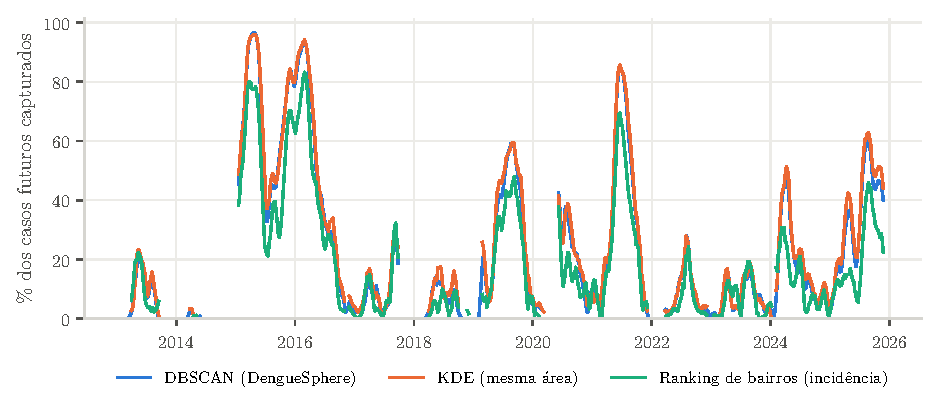
\includegraphics[width=\linewidth]{fig5_captura_temporal.pdf}
  \caption{Captura dos casos das 4 semanas seguintes ao longo do tempo (média móvel de 4 semanas; interrupções indicam
  semanas sem casos suficientes).}
  \label{fig:captura}
\end{figure}

\begin{figure}[htbp]
  \centering
  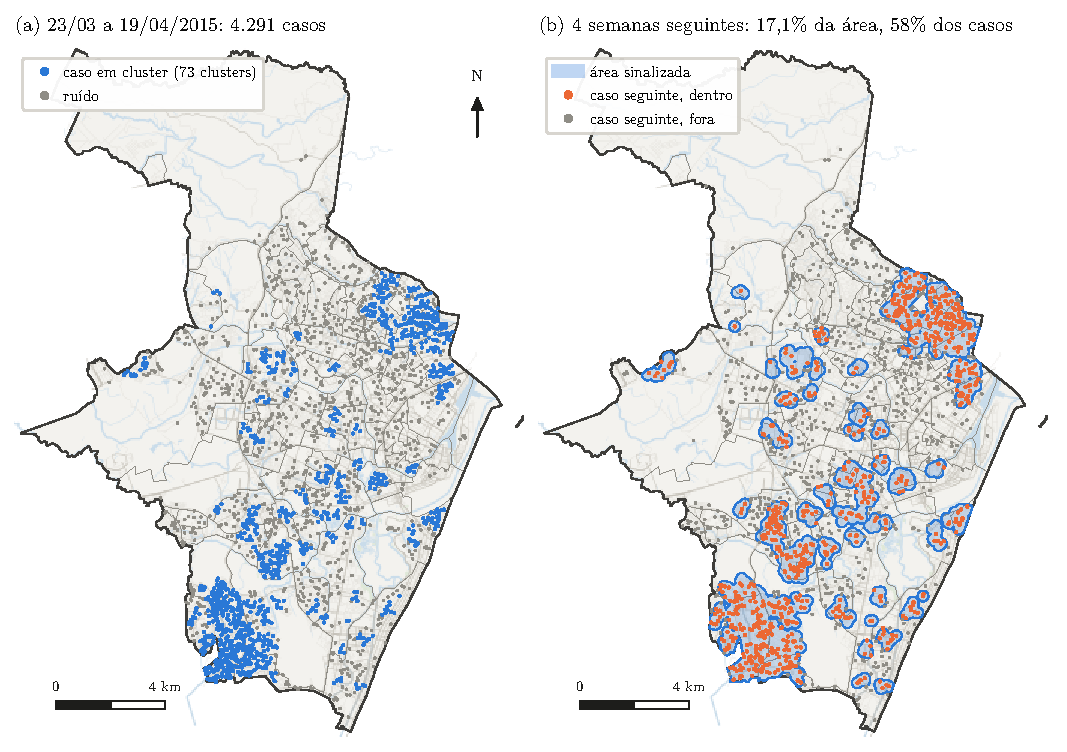
\includegraphics[width=\linewidth]{fig6_mapa_exemplo_2015.pdf}
  \caption{Exemplo de uso do DengueSphere no pico de 2015, com os parâmetros do estrato de alta incidência
  ($\varepsilon = 0{,}2$~km, \texttt{min\_samples} = 10). (a) Casos das quatro semanas analisadas: em azul, os
  atribuídos a algum cluster; em cinza, os classificados como ruído. (b) Área sinalizada (união dos círculos de raio
  $\varepsilon$ em torno dos casos em cluster) e casos ocorridos nas quatro semanas seguintes.}
  \label{fig:exemplo}
\end{figure}

A estratificação por incidência (\cref{tab:guia}) dá parâmetros práticos. Em baixa incidência, $\varepsilon = 0{,}5$~km e
\texttt{min\_samples} = 3 emitiram alerta em 99\% das janelas de teste, com PAI de 4,72 (praticamente igual ao da KDE,
4,85) e risco por habitante 2,21 vezes a média. Em alta incidência, $\varepsilon = 0{,}2$~km e \texttt{min\_samples} = 10 produziram áreas compactas (0,4\% do
município) com PAI de 6,15 e PAI$_\text{pop}$ de 2,34. No estrato intermediário, a configuração escolhida no treino ($\varepsilon = 0{,}2$~km,
\texttt{min\_samples} = 5) teve a taxa de alerta reduzida de 80\% para 62\% no teste, sinal de que esse estrato
demanda parâmetros menos restritivos.

\begin{table*}[htbp]
\centering
\small
\caption{Parâmetros escolhidos no treino para cada nível de incidência e seu desempenho no teste.}
\label{tab:guia}
\begin{adjustbox}{max width=\linewidth}
\begin{tabular}{lrrrrrrrrr}
\toprule
Incidência (casos/4 sem.) & $\varepsilon$ & min\_s. & Alerta treino \% & Alerta teste \% & PAI treino & PAI teste & PAI KDE teste & PAI$_\text{pop}$ teste & Área teste \% \\
\midrule
Baixa ($<$100) & 0,5 & 3 & 88 & 99 & 4,06 & 4,72 & 4,85 & 2,21 & 3,49 \\
Média (100--400) & 0,2 & 5 & 80 & 62 & 12,00 & 12,78 & 16,47 & 4,59 & 0,13 \\
Alta ($>$400) & 0,2 & 10 & 94 & 85 & 4,74 & 6,15 & 8,19 & 2,34 & 0,43 \\
\bottomrule
\end{tabular}
\end{adjustbox}
\par\smallskip\begin{minipage}{0.95\linewidth}\footnotesize Mesmo critério de escolha da Tabela~\ref{tab:grade}, aplicado dentro de cada estrato.\end{minipage}
\end{table*}


Os resultados se mantiveram quando a análise usou todas as notificações não descartadas, que é o que a vigilância
dispõe em tempo real (PAI 4,64 contra 4,79 e PAI$_\text{pop}$ 2,05 contra 2,14 na análise principal;
\cref{tab:variantes}). Incluir os casos localizados
apenas pelo centroide do bairro elevou o PAI para 5,33. Esse ganho, porém, é em parte artificial: casos empilhados no
mesmo ponto formam clusters densos.

\begin{table*}[htbp]
\centering
\small
\caption{Análise de sensibilidade da validação prospectiva (2013--2025, configuração principal; medianas nas janelas com alerta).}
\label{tab:variantes}
\begin{adjustbox}{max width=\linewidth}
\begin{tabular}{lrrrrrrrr}
\toprule
& & & & \multicolumn{2}{c}{DBSCAN} & \multicolumn{3}{c}{PAI$_\text{pop}$ das referências} \\
\cmidrule(lr){5-6}\cmidrule(lr){7-9}
Variante & Janelas & Alerta \% & Capt. \% & PAI & PAI$_\text{pop}$ & KDE & Bairros & População \\
\midrule
Principal: confirmados, nível de rua & 593 & 91 & 15,1 & 4,79 & 2,14 & 2,33 & 2,00 & 0,75 \\
Não descartados (tempo real), nível de rua & 595 & 91 & 15,1 & 4,64 & 2,05 & 2,26 & 1,90 & 0,78 \\
Confirmados, incluindo centroides de bairro & 606 & 95 & 17,6 & 5,33 & 2,41 & 2,68 & 2,17 & 0,78 \\
\bottomrule
\end{tabular}
\end{adjustbox}
\par\smallskip\begin{minipage}{0.95\linewidth}\footnotesize Não descartados: confirmados, inconclusivos e sem classificação final --- o conjunto disponível à vigilância antes do encerramento das investigações. Com centroides de bairro, casos empilhados no mesmo ponto formam clusters artificiais, o que infla a captura.\end{minipage}
\end{table*}


\subsection{Desempenho computacional}

A clusterização do DengueSphere processou \num{40000} casos em 0,35~s ($\varepsilon = 0{,}3$~km) e 0,50~s
($\varepsilon = 0{,}5$~km), com crescimento moderadamente superlinear no número de casos (40 vezes mais casos, cerca de 115 vezes mais tempo) (\cref{tab:desempenho}). Isso é
mais que o maior volume semanal observado (\num{1573} casos) e que o total do ano de 2015 (\num{23576}). Varreduras de
parâmetros como as deste estudo são, portanto, viáveis em tempo interativo.

\begin{table}[htbp]
\centering
\small
\caption{Tempo de execução da clusterização do DengueSphere (mediana de 3 execuções).}
\label{tab:desempenho}
\begin{adjustbox}{max width=\linewidth}
\begin{tabular}{rrr}
\toprule
Casos & eps = 0,3 km (ms) & eps = 0,5 km (ms) \\
\midrule
1.000 & 3 & 4 \\
2.500 & 9 & 12 \\
5.000 & 21 & 26 \\
10.000 & 55 & 71 \\
20.000 & 139 & 192 \\
40.000 & 350 & 499 \\
\bottomrule
\end{tabular}
\end{adjustbox}
\par\smallskip\begin{minipage}{0.95\linewidth}\footnotesize \texttt{executar\_clusterizacao} (DBSCAN, métrica haversine, \textit{ball tree}), min\_samples = 10; Apple M2, 16 GB, Python 3.11, scikit-learn.\end{minipage}
\end{table}


\section{Discussão}

Aplicado ao histórico de 13 anos do Recife, o DengueSphere sinaliza áreas que concentram os casos das semanas seguintes
cerca de cinco vezes mais do que o acaso por unidade de área e duas vezes mais do que a média por habitante. O
desempenho foi estável entre treino e teste, robusto a perturbações dos parâmetros e dos dados e mantido com as
notificações disponíveis em tempo real. O ajuste pela população do Censo 2022 é essencial para essa leitura. Sem ele,
seria possível atribuir ao software um mérito que é apenas da densidade demográfica; com ele, fica claro que as áreas
detectadas têm risco por habitante acima da média, enquanto as áreas simplesmente mais populosas têm risco abaixo dela.

A comparação com o ranking de bairros por incidência mostra onde está o ganho do DBSCAN. Por habitante, as duas
estratégias se equivalem; por área, o DBSCAN concentra o mesmo rendimento em cerca de metade do território. Como as
ações de controle vetorial (visitas domiciliares, eliminação de criadouros, bloqueio de transmissão) são planejadas por
território e quarteirão, delimitar agregados de algumas centenas de metros em vez de bairros inteiros reduz o esforço de
campo para um mesmo número de casos alcançados.

A KDE de mesma área obteve desempenho ligeiramente superior (diferença mediana de 0,36 no PAI e de 0,10 no
PAI$_\text{pop}$). Essa diferença deve ser lida à luz das funções distintas dos dois métodos. A KDE produz uma superfície
contínua que exige a escolha externa de um limiar de área. O DBSCAN decide por si quantos agregados existem e quais casos
são isolados, e entrega unidades discretas, enumeráveis e com contagem de casos, mais diretamente convertíveis em ordens
de serviço para as equipes de campo. A comparação mostra que esse ganho operacional custa pouca precisão preditiva, e o
resultado sugere incorporar ao software uma camada de densidade kernel complementar.

O achado com maior implicação prática é a dependência dos parâmetros em relação ao nível de incidência. Valores fixos
de \texttt{min\_samples} adequados a epidemias tornam o software mudo em períodos interepidêmicos, justamente quando a
detecção precoce de agregados é mais útil. As configurações da \cref{tab:guia} podem servir como valores padrão
adaptativos, selecionados automaticamente pelo número de casos da janela.

\paragraph{Limitações.} (i) A geocodificação usa uma base local do OpenStreetMap, e não o serviço Nominatim do software.
A concordância de 56~m (mediana) indica que isso não altera as conclusões em escala de bairro, mas logradouros ausentes
do OSM, sobretudo em áreas de ocupação informal, foram localizados pelo bairro e excluídos da análise principal
(17,1\% dos casos). (ii) Cerca de 90\% das confirmações foram por critério clínico-epidemiológico
(\cref{tab:classificacao}), e o segundo pico de 2015--2016 coincide com a epidemia de Zika no Recife, o que sugere
alguma má classificação entre arboviroses. (iii) A população do Censo 2022 foi usada para todos os anos e
distribuída dentro de cada setor censitário de modo uniforme (ponderação areal), o que ignora mudanças demográficas
intercensitárias e a distribuição interna das moradias. Além disso, a proporção de casos geocodificados no nível de rua
pode ser menor em áreas de ocupação informal, o que subestimaria a incidência justamente nas áreas mais vulneráveis. (iv) Faltam dados de agosto a dezembro de 2014. (v) A validação mede concentração espacial de casos
futuros, e não o efeito de intervenções, que só poderá ser avaliado com o uso operacional do software.

\appendix
\section{Material suplementar}
\begin{table}[htbp]
\centering
\small
\caption{Classificação final das notificações e critério de confirmação dos casos confirmados, por ano.}
\label{tab:classificacao}
\begin{adjustbox}{max width=\linewidth}
\begin{tabular}{lrrrrrr}
\toprule
Ano & Confirmados & Descartados & Inconclusivos & Sem classif. & Laboratorial (\%) & Clínico-epid. (\%) \\
\midrule
2013 & 1.304 & 1.958 & 0 & 0 & 11,9 & 88,1 \\
2014 & 363 & 796 & 0 & 0 & 20,4 & 79,6 \\
2015 & 23.576 & 7.913 & 3.178 & 8 & 7,3 & 92,1 \\
2016 & 12.083 & 4.884 & 1.515 & 23 & 2,0 & 95,3 \\
2017 & 955 & 1.486 & 4 & 0 & 6,7 & 93,3 \\
2018 & 1.207 & 1.466 & 13 & 0 & 15,2 & 84,8 \\
2019 & 4.102 & 2.606 & 601 & 0 & 10,6 & 89,4 \\
2020 & 1.544 & 1.952 & 122 & 1 & 7,2 & 90,7 \\
2021 & 7.435 & 3.541 & 1 & 0 & 6,3 & 93,7 \\
2022 & 1.291 & 1.503 & 1 & 0 & 7,6 & 92,4 \\
2023 & 1.414 & 2.004 & 83 & 1 & 2,5 & 96,7 \\
2024 & 3.007 & 7.231 & 119 & 126 & 3,2 & 78,1 \\
2025 & 5.066 & 3.452 & 286 & 247 & 16,6 & 73,8 \\
\bottomrule
\end{tabular}
\end{adjustbox}
\par\smallskip\begin{minipage}{0.95\linewidth}\footnotesize Confirmados: códigos 1--4 (classificação até 2014: dengue clássico, com complicações, FHD, SCD) e 10--12 (classificação de 2014: dengue, com sinais de alarme, grave).\end{minipage}
\end{table}


\begin{figure}[htbp]
  \centering
  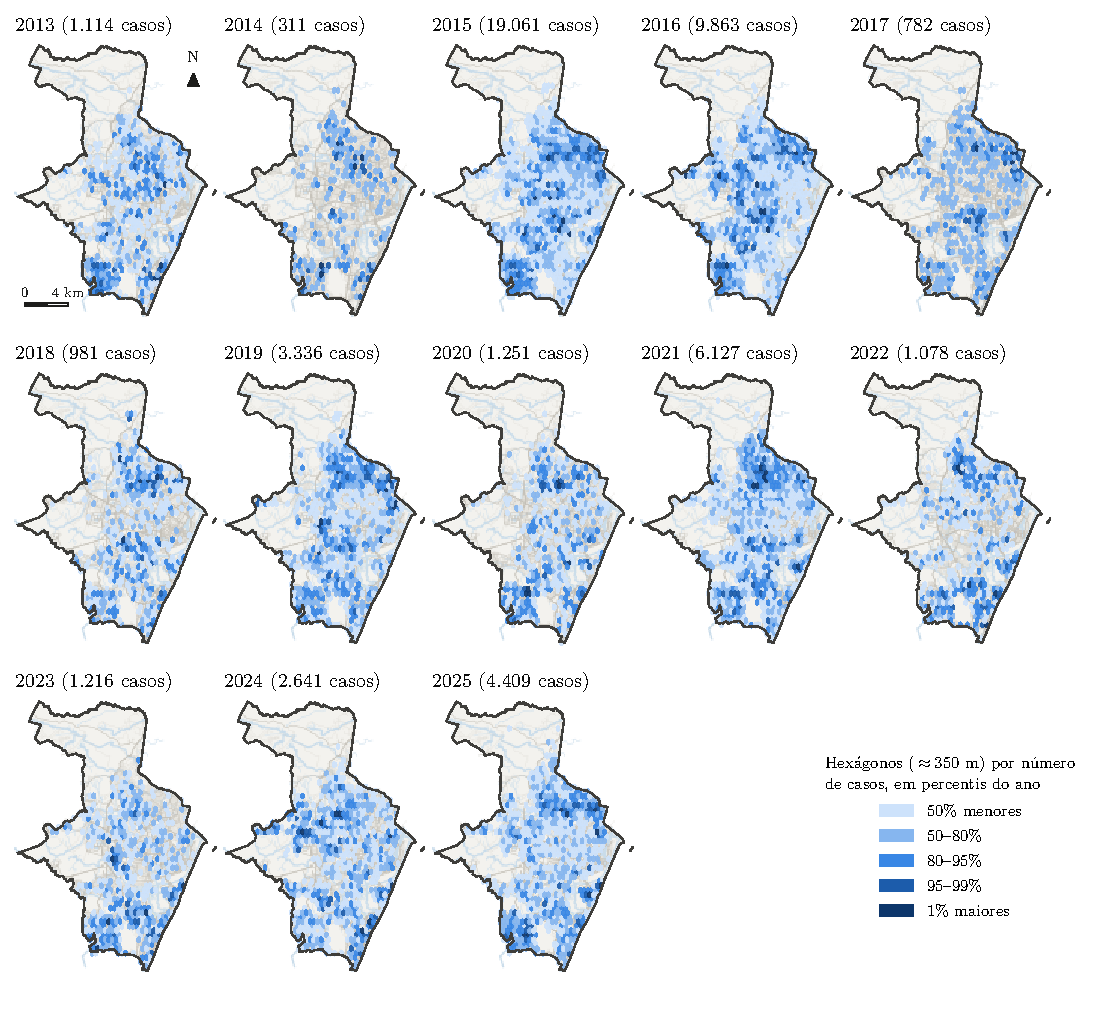
\includegraphics[width=\linewidth]{fig8_mapas_calor_anuais_todos_anos.pdf}
  \caption{Mapas de calor da distribuição dos casos confirmados em todos os anos do estudo (mesma construção da
  \cref{fig:mapas}). Em 2014 há dados apenas até julho.}
  \label{fig:mapas_todos}
\end{figure}

\begin{figure}[htbp]
  \centering
  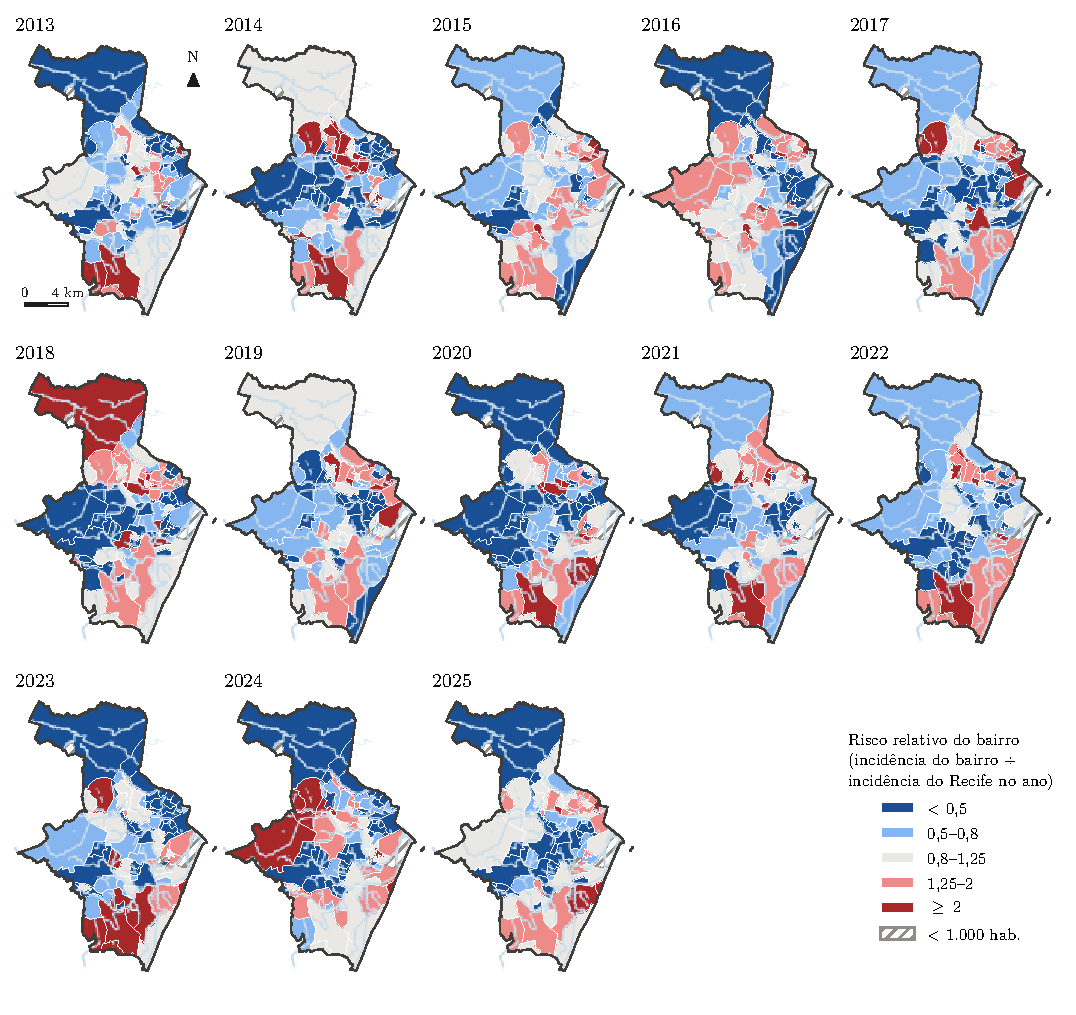
\includegraphics[width=\linewidth]{fig11_risco_relativo_bairros_todos_anos.pdf}
  \caption{Risco relativo de dengue por bairro em todos os anos do estudo (mesma construção da \cref{fig:rr}). Em
  anos de baixa incidência, bairros pouco populosos e extensos, como Guabiraba, alternam entre classes extremas por
  instabilidade da taxa.}
  \label{fig:rr_todos}
\end{figure}

\end{document}
